% !TEX encoding = UTF-8 Unicode
\documentclass[10pt]{standalone}\usepackage{tikz,graphicx}
\usepackage{fontspec}
\setmainfont{Arial}
\setsansfont{Arial}\begin{document}

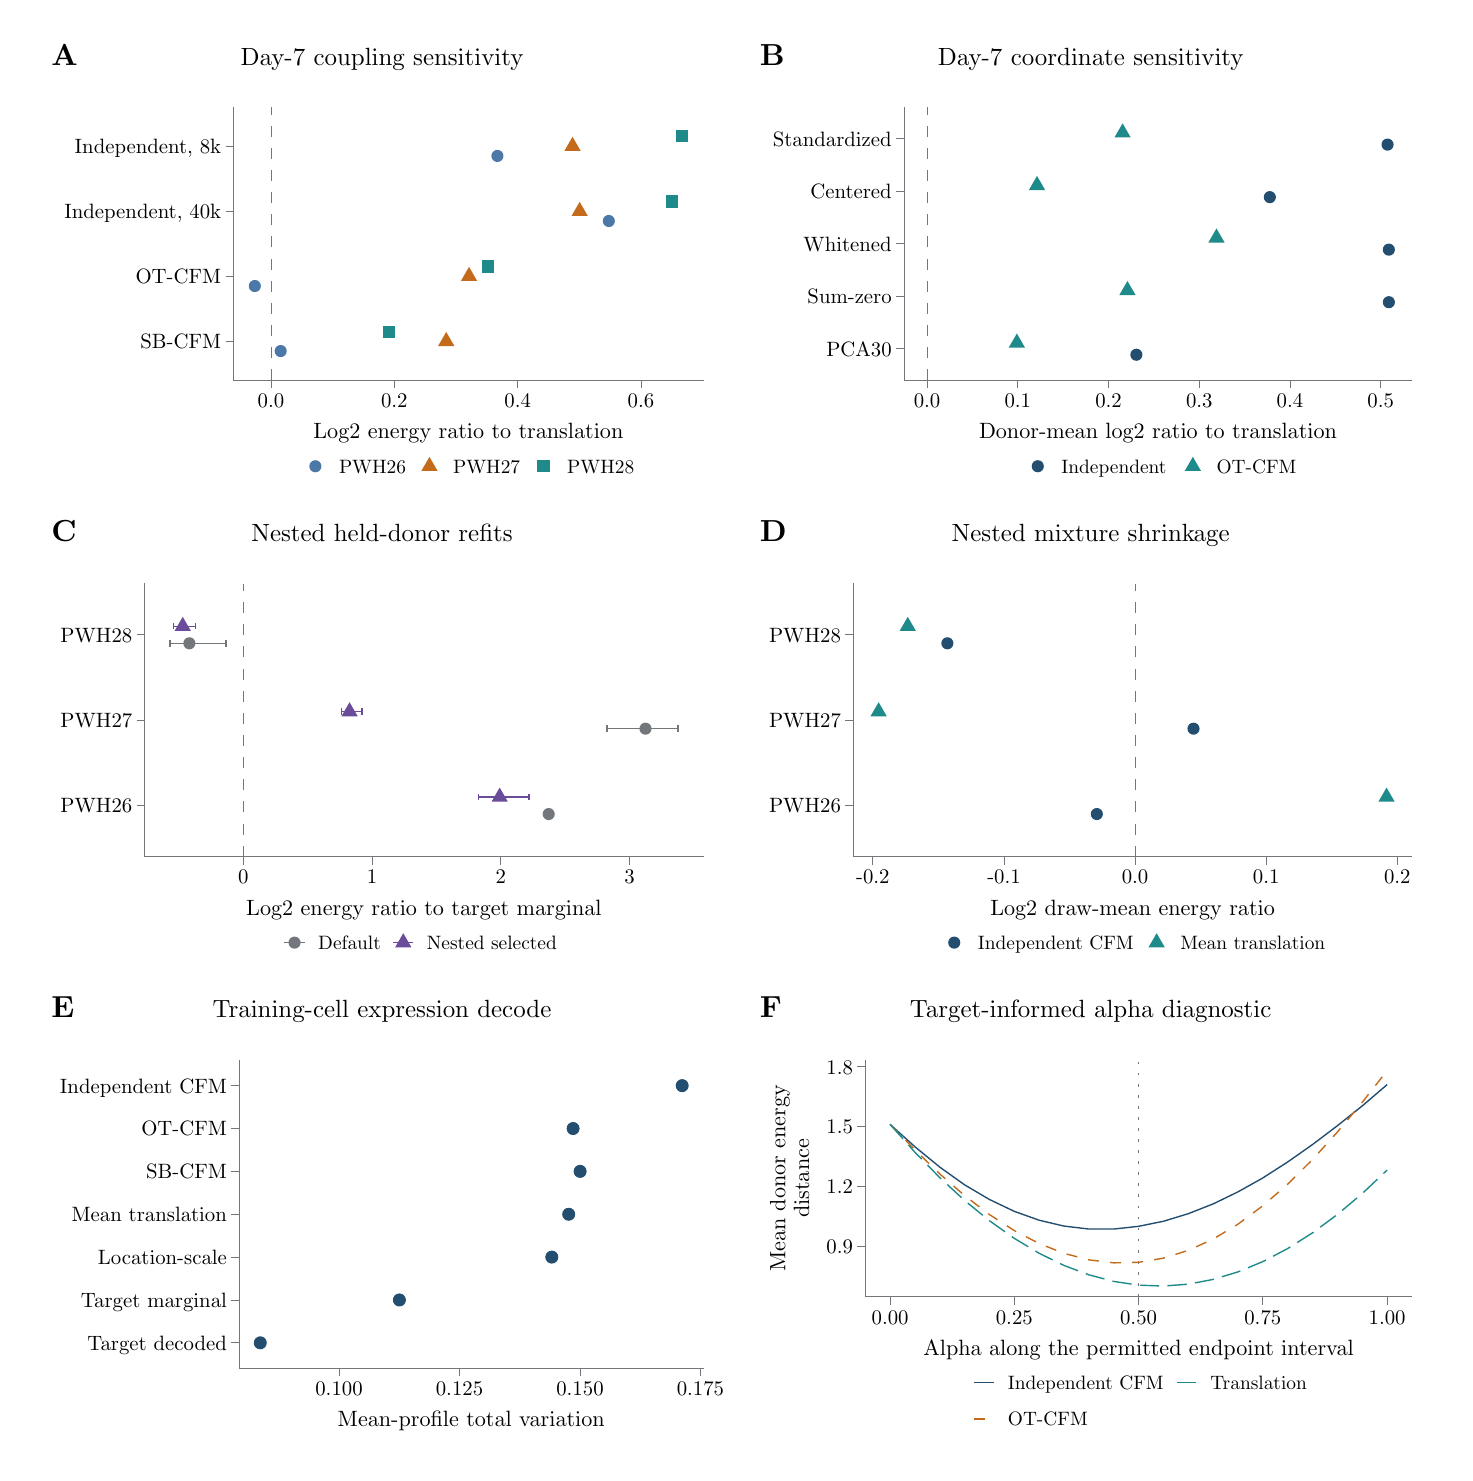
\begin{tikzpicture}[x=1pt,y=1pt]
\definecolor{fillColor}{RGB}{255,255,255}
\path[use as bounding box,fill=fillColor,fill opacity=0.00] (0,0) rectangle (512.15,514.99);
\begin{scope}
\path[clip] (  0.00,  0.00) rectangle (512.15,514.99);
\definecolor{drawColor}{RGB}{0,0,0}

\node[text=drawColor,anchor=base west,inner sep=0pt, outer sep=0pt, scale=  1.10] at (  8.54,501.43) {\bfseries A};

\node[text=drawColor,anchor=base,inner sep=0pt, outer sep=0pt, scale=  0.90] at (128.04,501.44) {Day-7 coupling sensitivity};
\end{scope}
\begin{scope}
\path[clip] (  8.54,348.55) rectangle (247.54,491.38);
\definecolor{fillColor}{RGB}{255,255,255}

\path[fill=fillColor] (  8.54,348.55) rectangle (247.54,491.38);
\end{scope}
\begin{scope}
\path[clip] ( 74.36,387.55) rectangle (244.12,486.26);
\definecolor{fillColor}{RGB}{255,255,255}

\path[fill=fillColor] ( 74.36,387.55) rectangle (244.12,486.26);
\definecolor{drawColor}{RGB}{115,119,123}

\path[draw=drawColor,line width= 0.3pt,dash pattern=on 4pt off 4pt ,line join=round] ( 87.90,387.55) -- ( 87.90,486.26);
\definecolor{fillColor}{RGB}{76,120,168}

\path[fill=fillColor] (169.74,468.63) circle (  2.19);

\path[fill=fillColor] (210.00,445.13) circle (  2.19);

\path[fill=fillColor] ( 82.08,421.63) circle (  2.19);

\path[fill=fillColor] ( 91.42,398.13) circle (  2.19);
\definecolor{fillColor}{RGB}{196,106,27}

\path[fill=fillColor] (196.89,475.56) --
	(199.83,470.46) --
	(193.94,470.46) --
	cycle;

\path[fill=fillColor] (199.46,452.05) --
	(202.41,446.95) --
	(196.52,446.95) --
	cycle;

\path[fill=fillColor] (159.49,428.55) --
	(162.43,423.45) --
	(156.54,423.45) --
	cycle;

\path[fill=fillColor] (151.24,405.05) --
	(154.19,399.95) --
	(148.30,399.95) --
	cycle;
\definecolor{fillColor}{RGB}{31,138,138}

\path[fill=fillColor] (234.22,473.50) --
	(238.59,473.50) --
	(238.59,477.87) --
	(234.22,477.87) --
	cycle;

\path[fill=fillColor] (230.50,449.99) --
	(234.87,449.99) --
	(234.87,454.37) --
	(230.50,454.37) --
	cycle;

\path[fill=fillColor] (164.02,426.49) --
	(168.39,426.49) --
	(168.39,430.86) --
	(164.02,430.86) --
	cycle;

\path[fill=fillColor] (128.43,402.99) --
	(132.81,402.99) --
	(132.81,407.36) --
	(128.43,407.36) --
	cycle;
\end{scope}
\begin{scope}
\path[clip] (  0.00,  0.00) rectangle (512.15,514.99);
\definecolor{drawColor}{RGB}{115,119,123}

\path[draw=drawColor,line width= 0.3pt,line join=round,line cap=rect] ( 74.36,387.55) --
	( 74.36,486.26);
\end{scope}
\begin{scope}
\path[clip] (  0.00,  0.00) rectangle (512.15,514.99);
\definecolor{drawColor}{RGB}{0,0,0}

\node[text=drawColor,anchor=base east,inner sep=0pt, outer sep=0pt, scale=  0.75] at ( 69.92,398.97) {SB-CFM};

\node[text=drawColor,anchor=base east,inner sep=0pt, outer sep=0pt, scale=  0.75] at ( 69.92,422.47) {OT-CFM};

\node[text=drawColor,anchor=base east,inner sep=0pt, outer sep=0pt, scale=  0.75] at ( 69.92,445.97) {Independent, 40k};

\node[text=drawColor,anchor=base east,inner sep=0pt, outer sep=0pt, scale=  0.75] at ( 69.92,469.47) {Independent, 8k};
\end{scope}
\begin{scope}
\path[clip] (  0.00,  0.00) rectangle (512.15,514.99);
\definecolor{drawColor}{RGB}{115,119,123}

\path[draw=drawColor,line width= 0.3pt,line join=round] ( 71.52,401.65) --
	( 74.36,401.65);

\path[draw=drawColor,line width= 0.3pt,line join=round] ( 71.52,425.15) --
	( 74.36,425.15);

\path[draw=drawColor,line width= 0.3pt,line join=round] ( 71.52,448.65) --
	( 74.36,448.65);

\path[draw=drawColor,line width= 0.3pt,line join=round] ( 71.52,472.16) --
	( 74.36,472.16);
\end{scope}
\begin{scope}
\path[clip] (  0.00,  0.00) rectangle (512.15,514.99);
\definecolor{drawColor}{RGB}{115,119,123}

\path[draw=drawColor,line width= 0.3pt,line join=round,line cap=rect] ( 74.36,387.55) --
	(244.12,387.55);
\end{scope}
\begin{scope}
\path[clip] (  0.00,  0.00) rectangle (512.15,514.99);
\definecolor{drawColor}{RGB}{115,119,123}

\path[draw=drawColor,line width= 0.3pt,line join=round] ( 87.90,384.70) --
	( 87.90,387.55);

\path[draw=drawColor,line width= 0.3pt,line join=round] (132.48,384.70) --
	(132.48,387.55);

\path[draw=drawColor,line width= 0.3pt,line join=round] (177.05,384.70) --
	(177.05,387.55);

\path[draw=drawColor,line width= 0.3pt,line join=round] (221.62,384.70) --
	(221.62,387.55);
\end{scope}
\begin{scope}
\path[clip] (  0.00,  0.00) rectangle (512.15,514.99);
\definecolor{drawColor}{RGB}{0,0,0}

\node[text=drawColor,anchor=base,inner sep=0pt, outer sep=0pt, scale=  0.75] at ( 87.90,377.74) {0.0};

\node[text=drawColor,anchor=base,inner sep=0pt, outer sep=0pt, scale=  0.75] at (132.48,377.74) {0.2};

\node[text=drawColor,anchor=base,inner sep=0pt, outer sep=0pt, scale=  0.75] at (177.05,377.74) {0.4};

\node[text=drawColor,anchor=base,inner sep=0pt, outer sep=0pt, scale=  0.75] at (221.62,377.74) {0.6};
\end{scope}
\begin{scope}
\path[clip] (  0.00,  0.00) rectangle (512.15,514.99);
\definecolor{drawColor}{RGB}{0,0,0}

\node[text=drawColor,anchor=base,inner sep=0pt, outer sep=0pt, scale=  0.80] at (159.24,366.45) {Log2 energy ratio to translation};
\end{scope}
\begin{scope}
\path[clip] (  0.00,  0.00) rectangle (512.15,514.99);
\definecolor{fillColor}{RGB}{255,255,255}

\path[fill=fillColor] ( 99.41,351.96) rectangle (219.08,361.07);
\end{scope}
\begin{scope}
\path[clip] (  0.00,  0.00) rectangle (512.15,514.99);
\definecolor{fillColor}{RGB}{255,255,255}

\path[fill=fillColor] ( 99.41,351.96) rectangle (108.52,361.07);
\definecolor{fillColor}{RGB}{76,120,168}

\path[fill=fillColor] (103.96,356.51) circle (  2.19);
\end{scope}
\begin{scope}
\path[clip] (  0.00,  0.00) rectangle (512.15,514.99);
\definecolor{fillColor}{RGB}{255,255,255}

\path[fill=fillColor] (140.63,351.96) rectangle (149.74,361.07);
\definecolor{fillColor}{RGB}{196,106,27}

\path[fill=fillColor] (145.19,359.91) --
	(148.13,354.81) --
	(142.24,354.81) --
	cycle;
\end{scope}
\begin{scope}
\path[clip] (  0.00,  0.00) rectangle (512.15,514.99);
\definecolor{fillColor}{RGB}{255,255,255}

\path[fill=fillColor] (181.85,351.96) rectangle (190.96,361.07);
\definecolor{fillColor}{RGB}{31,138,138}

\path[fill=fillColor] (184.22,354.33) --
	(188.59,354.33) --
	(188.59,358.70) --
	(184.22,358.70) --
	cycle;
\end{scope}
\begin{scope}
\path[clip] (  0.00,  0.00) rectangle (512.15,514.99);
\definecolor{drawColor}{RGB}{0,0,0}

\node[text=drawColor,anchor=base west,inner sep=0pt, outer sep=0pt, scale=  0.70] at (112.52,354.01) {PWH26};
\end{scope}
\begin{scope}
\path[clip] (  0.00,  0.00) rectangle (512.15,514.99);
\definecolor{drawColor}{RGB}{0,0,0}

\node[text=drawColor,anchor=base west,inner sep=0pt, outer sep=0pt, scale=  0.70] at (153.74,354.01) {PWH27};
\end{scope}
\begin{scope}
\path[clip] (  0.00,  0.00) rectangle (512.15,514.99);
\definecolor{drawColor}{RGB}{0,0,0}

\node[text=drawColor,anchor=base west,inner sep=0pt, outer sep=0pt, scale=  0.70] at (194.96,354.01) {PWH28};
\end{scope}
\begin{scope}
\path[clip] (  0.00,  0.00) rectangle (512.15,514.99);
\definecolor{drawColor}{RGB}{0,0,0}

\node[text=drawColor,anchor=base west,inner sep=0pt, outer sep=0pt, scale=  1.10] at (264.61,501.43) {\bfseries B};

\node[text=drawColor,anchor=base,inner sep=0pt, outer sep=0pt, scale=  0.90] at (384.11,501.44) {Day-7 coordinate sensitivity};
\end{scope}
\begin{scope}
\path[clip] (264.61,348.55) rectangle (503.61,491.38);
\definecolor{fillColor}{RGB}{255,255,255}

\path[fill=fillColor] (264.61,348.55) rectangle (503.61,491.38);
\end{scope}
\begin{scope}
\path[clip] (316.67,387.55) rectangle (500.20,486.26);
\definecolor{fillColor}{RGB}{255,255,255}

\path[fill=fillColor] (316.67,387.55) rectangle (500.20,486.26);
\definecolor{drawColor}{RGB}{115,119,123}

\path[draw=drawColor,line width= 0.3pt,dash pattern=on 4pt off 4pt ,line join=round] (325.01,387.55) -- (325.01,486.26);
\definecolor{fillColor}{RGB}{35,78,112}

\path[fill=fillColor] (491.86,415.79) circle (  2.19);
\definecolor{fillColor}{RGB}{31,138,138}

\path[fill=fillColor] (397.40,423.46) --
	(400.34,418.36) --
	(394.45,418.36) --
	cycle;
\definecolor{fillColor}{RGB}{35,78,112}

\path[fill=fillColor] (448.85,453.75) circle (  2.19);
\definecolor{fillColor}{RGB}{31,138,138}

\path[fill=fillColor] (364.72,461.42) --
	(367.67,456.32) --
	(361.78,456.32) --
	cycle;
\definecolor{fillColor}{RGB}{35,78,112}

\path[fill=fillColor] (491.39,472.73) circle (  2.19);
\definecolor{fillColor}{RGB}{31,138,138}

\path[fill=fillColor] (395.65,480.40) --
	(398.59,475.30) --
	(392.70,475.30) --
	cycle;
\definecolor{fillColor}{RGB}{35,78,112}

\path[fill=fillColor] (491.85,434.77) circle (  2.19);
\definecolor{fillColor}{RGB}{31,138,138}

\path[fill=fillColor] (429.57,442.44) --
	(432.52,437.34) --
	(426.63,437.34) --
	cycle;
\definecolor{fillColor}{RGB}{35,78,112}

\path[fill=fillColor] (400.63,396.80) circle (  2.19);
\definecolor{fillColor}{RGB}{31,138,138}

\path[fill=fillColor] (357.44,404.48) --
	(360.38,399.37) --
	(354.49,399.37) --
	cycle;
\end{scope}
\begin{scope}
\path[clip] (  0.00,  0.00) rectangle (512.15,514.99);
\definecolor{drawColor}{RGB}{115,119,123}

\path[draw=drawColor,line width= 0.3pt,line join=round,line cap=rect] (316.67,387.55) --
	(316.67,486.26);
\end{scope}
\begin{scope}
\path[clip] (  0.00,  0.00) rectangle (512.15,514.99);
\definecolor{drawColor}{RGB}{0,0,0}

\node[text=drawColor,anchor=base east,inner sep=0pt, outer sep=0pt, scale=  0.75] at (312.22,396.26) {PCA30};

\node[text=drawColor,anchor=base east,inner sep=0pt, outer sep=0pt, scale=  0.75] at (312.22,415.24) {Sum-zero};

\node[text=drawColor,anchor=base east,inner sep=0pt, outer sep=0pt, scale=  0.75] at (312.22,434.22) {Whitened};

\node[text=drawColor,anchor=base east,inner sep=0pt, outer sep=0pt, scale=  0.75] at (312.22,453.20) {Centered};

\node[text=drawColor,anchor=base east,inner sep=0pt, outer sep=0pt, scale=  0.75] at (312.22,472.18) {Standardized};
\end{scope}
\begin{scope}
\path[clip] (  0.00,  0.00) rectangle (512.15,514.99);
\definecolor{drawColor}{RGB}{115,119,123}

\path[draw=drawColor,line width= 0.3pt,line join=round] (313.82,398.94) --
	(316.67,398.94);

\path[draw=drawColor,line width= 0.3pt,line join=round] (313.82,417.92) --
	(316.67,417.92);

\path[draw=drawColor,line width= 0.3pt,line join=round] (313.82,436.90) --
	(316.67,436.90);

\path[draw=drawColor,line width= 0.3pt,line join=round] (313.82,455.89) --
	(316.67,455.89);

\path[draw=drawColor,line width= 0.3pt,line join=round] (313.82,474.87) --
	(316.67,474.87);
\end{scope}
\begin{scope}
\path[clip] (  0.00,  0.00) rectangle (512.15,514.99);
\definecolor{drawColor}{RGB}{115,119,123}

\path[draw=drawColor,line width= 0.3pt,line join=round,line cap=rect] (316.67,387.55) --
	(500.20,387.55);
\end{scope}
\begin{scope}
\path[clip] (  0.00,  0.00) rectangle (512.15,514.99);
\definecolor{drawColor}{RGB}{115,119,123}

\path[draw=drawColor,line width= 0.3pt,line join=round] (325.01,384.70) --
	(325.01,387.55);

\path[draw=drawColor,line width= 0.3pt,line join=round] (357.79,384.70) --
	(357.79,387.55);

\path[draw=drawColor,line width= 0.3pt,line join=round] (390.58,384.70) --
	(390.58,387.55);

\path[draw=drawColor,line width= 0.3pt,line join=round] (423.36,384.70) --
	(423.36,387.55);

\path[draw=drawColor,line width= 0.3pt,line join=round] (456.14,384.70) --
	(456.14,387.55);

\path[draw=drawColor,line width= 0.3pt,line join=round] (488.93,384.70) --
	(488.93,387.55);
\end{scope}
\begin{scope}
\path[clip] (  0.00,  0.00) rectangle (512.15,514.99);
\definecolor{drawColor}{RGB}{0,0,0}

\node[text=drawColor,anchor=base,inner sep=0pt, outer sep=0pt, scale=  0.75] at (325.01,377.74) {0.0};

\node[text=drawColor,anchor=base,inner sep=0pt, outer sep=0pt, scale=  0.75] at (357.79,377.74) {0.1};

\node[text=drawColor,anchor=base,inner sep=0pt, outer sep=0pt, scale=  0.75] at (390.58,377.74) {0.2};

\node[text=drawColor,anchor=base,inner sep=0pt, outer sep=0pt, scale=  0.75] at (423.36,377.74) {0.3};

\node[text=drawColor,anchor=base,inner sep=0pt, outer sep=0pt, scale=  0.75] at (456.14,377.74) {0.4};

\node[text=drawColor,anchor=base,inner sep=0pt, outer sep=0pt, scale=  0.75] at (488.93,377.74) {0.5};
\end{scope}
\begin{scope}
\path[clip] (  0.00,  0.00) rectangle (512.15,514.99);
\definecolor{drawColor}{RGB}{0,0,0}

\node[text=drawColor,anchor=base,inner sep=0pt, outer sep=0pt, scale=  0.80] at (408.43,366.45) {Donor-mean log2 ratio to translation};
\end{scope}
\begin{scope}
\path[clip] (  0.00,  0.00) rectangle (512.15,514.99);
\definecolor{fillColor}{RGB}{255,255,255}

\path[fill=fillColor] (360.45,351.96) rectangle (456.42,361.07);
\end{scope}
\begin{scope}
\path[clip] (  0.00,  0.00) rectangle (512.15,514.99);
\definecolor{fillColor}{RGB}{255,255,255}

\path[fill=fillColor] (360.45,351.96) rectangle (369.56,361.07);
\definecolor{fillColor}{RGB}{35,78,112}

\path[fill=fillColor] (365.00,356.51) circle (  2.19);
\end{scope}
\begin{scope}
\path[clip] (  0.00,  0.00) rectangle (512.15,514.99);
\definecolor{fillColor}{RGB}{255,255,255}

\path[fill=fillColor] (416.48,351.96) rectangle (425.59,361.07);
\definecolor{fillColor}{RGB}{31,138,138}

\path[fill=fillColor] (421.04,359.91) --
	(423.98,354.81) --
	(418.09,354.81) --
	cycle;
\end{scope}
\begin{scope}
\path[clip] (  0.00,  0.00) rectangle (512.15,514.99);
\definecolor{drawColor}{RGB}{0,0,0}

\node[text=drawColor,anchor=base west,inner sep=0pt, outer sep=0pt, scale=  0.70] at (373.56,354.01) {Independent};
\end{scope}
\begin{scope}
\path[clip] (  0.00,  0.00) rectangle (512.15,514.99);
\definecolor{drawColor}{RGB}{0,0,0}

\node[text=drawColor,anchor=base west,inner sep=0pt, outer sep=0pt, scale=  0.70] at (429.59,354.01) {OT-CFM};
\end{scope}
\begin{scope}
\path[clip] (  0.00,  0.00) rectangle (512.15,514.99);
\definecolor{drawColor}{RGB}{0,0,0}

\node[text=drawColor,anchor=base west,inner sep=0pt, outer sep=0pt, scale=  1.10] at (  8.54,329.29) {\bfseries C};

\node[text=drawColor,anchor=base,inner sep=0pt, outer sep=0pt, scale=  0.90] at (128.04,329.30) {Nested held-donor refits};
\end{scope}
\begin{scope}
\path[clip] (  8.54,176.41) rectangle (247.54,319.24);
\definecolor{fillColor}{RGB}{255,255,255}

\path[fill=fillColor] (  8.54,176.41) rectangle (247.54,319.24);
\end{scope}
\begin{scope}
\path[clip] ( 42.24,215.41) rectangle (244.12,314.12);
\definecolor{fillColor}{RGB}{255,255,255}

\path[fill=fillColor] ( 42.24,215.41) rectangle (244.12,314.12);
\definecolor{drawColor}{RGB}{115,119,123}

\path[draw=drawColor,line width= 0.3pt,dash pattern=on 4pt off 4pt ,line join=round] ( 77.95,215.41) -- ( 77.95,314.12);

\path[draw=drawColor,line width= 0.5pt,line join=round] (190.08,229.68) --
	(190.08,231.99);

\path[draw=drawColor,line width= 0.5pt,line join=round] (190.08,230.83) --
	(186.91,230.83);

\path[draw=drawColor,line width= 0.5pt,line join=round] (186.91,229.68) --
	(186.91,231.99);
\definecolor{drawColor}{RGB}{107,76,154}

\path[draw=drawColor,line width= 0.5pt,line join=round] (181.15,235.85) --
	(181.15,238.16);

\path[draw=drawColor,line width= 0.5pt,line join=round] (181.15,237.00) --
	(162.86,237.00);

\path[draw=drawColor,line width= 0.5pt,line join=round] (162.86,235.85) --
	(162.86,238.16);
\definecolor{drawColor}{RGB}{115,119,123}

\path[draw=drawColor,line width= 0.5pt,line join=round] (234.95,260.52) --
	(234.95,262.84);

\path[draw=drawColor,line width= 0.5pt,line join=round] (234.95,261.68) --
	(209.35,261.68);

\path[draw=drawColor,line width= 0.5pt,line join=round] (209.35,260.52) --
	(209.35,262.84);
\definecolor{drawColor}{RGB}{107,76,154}

\path[draw=drawColor,line width= 0.5pt,line join=round] (120.76,266.69) --
	(120.76,269.01);

\path[draw=drawColor,line width= 0.5pt,line join=round] (120.76,267.85) --
	(113.40,267.85);

\path[draw=drawColor,line width= 0.5pt,line join=round] (113.40,266.69) --
	(113.40,269.01);
\definecolor{drawColor}{RGB}{115,119,123}

\path[draw=drawColor,line width= 0.5pt,line join=round] ( 71.66,291.37) --
	( 71.66,293.68);

\path[draw=drawColor,line width= 0.5pt,line join=round] ( 71.66,292.53) --
	( 51.41,292.53);

\path[draw=drawColor,line width= 0.5pt,line join=round] ( 51.41,291.37) --
	( 51.41,293.68);
\definecolor{drawColor}{RGB}{107,76,154}

\path[draw=drawColor,line width= 0.5pt,line join=round] ( 60.68,297.54) --
	( 60.68,299.85);

\path[draw=drawColor,line width= 0.5pt,line join=round] ( 60.68,298.70) --
	( 52.64,298.70);

\path[draw=drawColor,line width= 0.5pt,line join=round] ( 52.64,297.54) --
	( 52.64,299.85);
\definecolor{fillColor}{RGB}{115,119,123}

\path[fill=fillColor] (188.27,230.83) circle (  2.19);
\definecolor{fillColor}{RGB}{107,76,154}

\path[fill=fillColor] (170.56,240.40) --
	(173.51,235.30) --
	(167.62,235.30) --
	cycle;
\definecolor{fillColor}{RGB}{115,119,123}

\path[fill=fillColor] (223.24,261.68) circle (  2.19);
\definecolor{fillColor}{RGB}{107,76,154}

\path[fill=fillColor] (116.31,271.25) --
	(119.26,266.15) --
	(113.37,266.15) --
	cycle;
\definecolor{fillColor}{RGB}{115,119,123}

\path[fill=fillColor] ( 58.43,292.53) circle (  2.19);
\definecolor{fillColor}{RGB}{107,76,154}

\path[fill=fillColor] ( 56.03,302.10) --
	( 58.97,297.00) --
	( 53.08,297.00) --
	cycle;
\end{scope}
\begin{scope}
\path[clip] (  0.00,  0.00) rectangle (512.15,514.99);
\definecolor{drawColor}{RGB}{115,119,123}

\path[draw=drawColor,line width= 0.3pt,line join=round,line cap=rect] ( 42.24,215.41) --
	( 42.24,314.12);
\end{scope}
\begin{scope}
\path[clip] (  0.00,  0.00) rectangle (512.15,514.99);
\definecolor{drawColor}{RGB}{0,0,0}

\node[text=drawColor,anchor=base east,inner sep=0pt, outer sep=0pt, scale=  0.75] at ( 37.79,231.23) {PWH26};

\node[text=drawColor,anchor=base east,inner sep=0pt, outer sep=0pt, scale=  0.75] at ( 37.79,262.08) {PWH27};

\node[text=drawColor,anchor=base east,inner sep=0pt, outer sep=0pt, scale=  0.75] at ( 37.79,292.93) {PWH28};
\end{scope}
\begin{scope}
\path[clip] (  0.00,  0.00) rectangle (512.15,514.99);
\definecolor{drawColor}{RGB}{115,119,123}

\path[draw=drawColor,line width= 0.3pt,line join=round] ( 39.39,233.92) --
	( 42.24,233.92);

\path[draw=drawColor,line width= 0.3pt,line join=round] ( 39.39,264.76) --
	( 42.24,264.76);

\path[draw=drawColor,line width= 0.3pt,line join=round] ( 39.39,295.61) --
	( 42.24,295.61);
\end{scope}
\begin{scope}
\path[clip] (  0.00,  0.00) rectangle (512.15,514.99);
\definecolor{drawColor}{RGB}{115,119,123}

\path[draw=drawColor,line width= 0.3pt,line join=round,line cap=rect] ( 42.24,215.41) --
	(244.12,215.41);
\end{scope}
\begin{scope}
\path[clip] (  0.00,  0.00) rectangle (512.15,514.99);
\definecolor{drawColor}{RGB}{115,119,123}

\path[draw=drawColor,line width= 0.3pt,line join=round] ( 77.95,212.57) --
	( 77.95,215.41);

\path[draw=drawColor,line width= 0.3pt,line join=round] (124.47,212.57) --
	(124.47,215.41);

\path[draw=drawColor,line width= 0.3pt,line join=round] (170.99,212.57) --
	(170.99,215.41);

\path[draw=drawColor,line width= 0.3pt,line join=round] (217.51,212.57) --
	(217.51,215.41);
\end{scope}
\begin{scope}
\path[clip] (  0.00,  0.00) rectangle (512.15,514.99);
\definecolor{drawColor}{RGB}{0,0,0}

\node[text=drawColor,anchor=base,inner sep=0pt, outer sep=0pt, scale=  0.75] at ( 77.95,205.60) {0};

\node[text=drawColor,anchor=base,inner sep=0pt, outer sep=0pt, scale=  0.75] at (124.47,205.60) {1};

\node[text=drawColor,anchor=base,inner sep=0pt, outer sep=0pt, scale=  0.75] at (170.99,205.60) {2};

\node[text=drawColor,anchor=base,inner sep=0pt, outer sep=0pt, scale=  0.75] at (217.51,205.60) {3};
\end{scope}
\begin{scope}
\path[clip] (  0.00,  0.00) rectangle (512.15,514.99);
\definecolor{drawColor}{RGB}{0,0,0}

\node[text=drawColor,anchor=base,inner sep=0pt, outer sep=0pt, scale=  0.80] at (143.18,194.31) {Log2 energy ratio to target marginal};
\end{scope}
\begin{scope}
\path[clip] (  0.00,  0.00) rectangle (512.15,514.99);
\definecolor{fillColor}{RGB}{255,255,255}

\path[fill=fillColor] ( 91.89,179.82) rectangle (194.47,188.93);
\end{scope}
\begin{scope}
\path[clip] (  0.00,  0.00) rectangle (512.15,514.99);
\definecolor{fillColor}{RGB}{255,255,255}

\path[fill=fillColor] ( 91.89,179.82) rectangle (100.99,188.93);
\definecolor{drawColor}{RGB}{115,119,123}

\path[draw=drawColor,line width= 0.5pt,line join=round] ( 92.80,184.37) -- (100.08,184.37);
\definecolor{fillColor}{RGB}{115,119,123}

\path[fill=fillColor] ( 96.44,184.37) circle (  2.19);
\end{scope}
\begin{scope}
\path[clip] (  0.00,  0.00) rectangle (512.15,514.99);
\definecolor{fillColor}{RGB}{255,255,255}

\path[fill=fillColor] (131.17,179.82) rectangle (140.28,188.93);
\definecolor{drawColor}{RGB}{107,76,154}

\path[draw=drawColor,line width= 0.5pt,line join=round] (132.08,184.37) -- (139.37,184.37);
\definecolor{fillColor}{RGB}{107,76,154}

\path[fill=fillColor] (135.72,187.77) --
	(138.67,182.67) --
	(132.78,182.67) --
	cycle;
\end{scope}
\begin{scope}
\path[clip] (  0.00,  0.00) rectangle (512.15,514.99);
\definecolor{drawColor}{RGB}{0,0,0}

\node[text=drawColor,anchor=base west,inner sep=0pt, outer sep=0pt, scale=  0.70] at (104.99,181.87) {Default};
\end{scope}
\begin{scope}
\path[clip] (  0.00,  0.00) rectangle (512.15,514.99);
\definecolor{drawColor}{RGB}{0,0,0}

\node[text=drawColor,anchor=base west,inner sep=0pt, outer sep=0pt, scale=  0.70] at (144.28,181.87) {Nested selected};
\end{scope}
\begin{scope}
\path[clip] (  0.00,  0.00) rectangle (512.15,514.99);
\definecolor{drawColor}{RGB}{0,0,0}

\node[text=drawColor,anchor=base west,inner sep=0pt, outer sep=0pt, scale=  1.10] at (264.61,329.29) {\bfseries D};

\node[text=drawColor,anchor=base,inner sep=0pt, outer sep=0pt, scale=  0.90] at (384.11,329.30) {Nested mixture shrinkage};
\end{scope}
\begin{scope}
\path[clip] (264.61,176.41) rectangle (503.61,319.24);
\definecolor{fillColor}{RGB}{255,255,255}

\path[fill=fillColor] (264.61,176.41) rectangle (503.61,319.24);
\end{scope}
\begin{scope}
\path[clip] (298.31,215.41) rectangle (500.20,314.12);
\definecolor{fillColor}{RGB}{255,255,255}

\path[fill=fillColor] (298.31,215.41) rectangle (500.20,314.12);
\definecolor{drawColor}{RGB}{115,119,123}

\path[draw=drawColor,line width= 0.3pt,dash pattern=on 4pt off 4pt ,line join=round] (400.16,215.41) -- (400.16,314.12);
\definecolor{fillColor}{RGB}{35,78,112}

\path[fill=fillColor] (386.33,230.83) circle (  2.19);

\path[fill=fillColor] (421.27,261.68) circle (  2.19);

\path[fill=fillColor] (332.33,292.53) circle (  2.19);
\definecolor{fillColor}{RGB}{31,138,138}

\path[fill=fillColor] (491.02,240.40) --
	(493.97,235.30) --
	(488.08,235.30) --
	cycle;

\path[fill=fillColor] (307.49,271.25) --
	(310.43,266.15) --
	(304.54,266.15) --
	cycle;

\path[fill=fillColor] (318.02,302.10) --
	(320.96,297.00) --
	(315.07,297.00) --
	cycle;
\end{scope}
\begin{scope}
\path[clip] (  0.00,  0.00) rectangle (512.15,514.99);
\definecolor{drawColor}{RGB}{115,119,123}

\path[draw=drawColor,line width= 0.3pt,line join=round,line cap=rect] (298.31,215.41) --
	(298.31,314.12);
\end{scope}
\begin{scope}
\path[clip] (  0.00,  0.00) rectangle (512.15,514.99);
\definecolor{drawColor}{RGB}{0,0,0}

\node[text=drawColor,anchor=base east,inner sep=0pt, outer sep=0pt, scale=  0.75] at (293.86,231.23) {PWH26};

\node[text=drawColor,anchor=base east,inner sep=0pt, outer sep=0pt, scale=  0.75] at (293.86,262.08) {PWH27};

\node[text=drawColor,anchor=base east,inner sep=0pt, outer sep=0pt, scale=  0.75] at (293.86,292.93) {PWH28};
\end{scope}
\begin{scope}
\path[clip] (  0.00,  0.00) rectangle (512.15,514.99);
\definecolor{drawColor}{RGB}{115,119,123}

\path[draw=drawColor,line width= 0.3pt,line join=round] (295.46,233.92) --
	(298.31,233.92);

\path[draw=drawColor,line width= 0.3pt,line join=round] (295.46,264.76) --
	(298.31,264.76);

\path[draw=drawColor,line width= 0.3pt,line join=round] (295.46,295.61) --
	(298.31,295.61);
\end{scope}
\begin{scope}
\path[clip] (  0.00,  0.00) rectangle (512.15,514.99);
\definecolor{drawColor}{RGB}{115,119,123}

\path[draw=drawColor,line width= 0.3pt,line join=round,line cap=rect] (298.31,215.41) --
	(500.20,215.41);
\end{scope}
\begin{scope}
\path[clip] (  0.00,  0.00) rectangle (512.15,514.99);
\definecolor{drawColor}{RGB}{115,119,123}

\path[draw=drawColor,line width= 0.3pt,line join=round] (305.41,212.57) --
	(305.41,215.41);

\path[draw=drawColor,line width= 0.3pt,line join=round] (352.79,212.57) --
	(352.79,215.41);

\path[draw=drawColor,line width= 0.3pt,line join=round] (400.16,212.57) --
	(400.16,215.41);

\path[draw=drawColor,line width= 0.3pt,line join=round] (447.54,212.57) --
	(447.54,215.41);

\path[draw=drawColor,line width= 0.3pt,line join=round] (494.92,212.57) --
	(494.92,215.41);
\end{scope}
\begin{scope}
\path[clip] (  0.00,  0.00) rectangle (512.15,514.99);
\definecolor{drawColor}{RGB}{0,0,0}

\node[text=drawColor,anchor=base,inner sep=0pt, outer sep=0pt, scale=  0.75] at (305.41,205.60) {-0.2};

\node[text=drawColor,anchor=base,inner sep=0pt, outer sep=0pt, scale=  0.75] at (352.79,205.60) {-0.1};

\node[text=drawColor,anchor=base,inner sep=0pt, outer sep=0pt, scale=  0.75] at (400.16,205.60) {0.0};

\node[text=drawColor,anchor=base,inner sep=0pt, outer sep=0pt, scale=  0.75] at (447.54,205.60) {0.1};

\node[text=drawColor,anchor=base,inner sep=0pt, outer sep=0pt, scale=  0.75] at (494.92,205.60) {0.2};
\end{scope}
\begin{scope}
\path[clip] (  0.00,  0.00) rectangle (512.15,514.99);
\definecolor{drawColor}{RGB}{0,0,0}

\node[text=drawColor,anchor=base,inner sep=0pt, outer sep=0pt, scale=  0.80] at (399.25,194.31) {Log2 draw-mean energy ratio};
\end{scope}
\begin{scope}
\path[clip] (  0.00,  0.00) rectangle (512.15,514.99);
\definecolor{fillColor}{RGB}{255,255,255}

\path[fill=fillColor] (330.26,179.82) rectangle (468.25,188.93);
\end{scope}
\begin{scope}
\path[clip] (  0.00,  0.00) rectangle (512.15,514.99);
\definecolor{fillColor}{RGB}{255,255,255}

\path[fill=fillColor] (330.26,179.82) rectangle (339.36,188.93);
\definecolor{fillColor}{RGB}{35,78,112}

\path[fill=fillColor] (334.81,184.37) circle (  2.19);
\end{scope}
\begin{scope}
\path[clip] (  0.00,  0.00) rectangle (512.15,514.99);
\definecolor{fillColor}{RGB}{255,255,255}

\path[fill=fillColor] (403.40,179.82) rectangle (412.50,188.93);
\definecolor{fillColor}{RGB}{31,138,138}

\path[fill=fillColor] (407.95,187.77) --
	(410.89,182.67) --
	(405.00,182.67) --
	cycle;
\end{scope}
\begin{scope}
\path[clip] (  0.00,  0.00) rectangle (512.15,514.99);
\definecolor{drawColor}{RGB}{0,0,0}

\node[text=drawColor,anchor=base west,inner sep=0pt, outer sep=0pt, scale=  0.70] at (343.36,181.87) {Independent CFM};
\end{scope}
\begin{scope}
\path[clip] (  0.00,  0.00) rectangle (512.15,514.99);
\definecolor{drawColor}{RGB}{0,0,0}

\node[text=drawColor,anchor=base west,inner sep=0pt, outer sep=0pt, scale=  0.70] at (416.50,181.87) {Mean translation};
\end{scope}
\begin{scope}
\path[clip] (  0.00,  0.00) rectangle (512.15,514.99);
\definecolor{drawColor}{RGB}{0,0,0}

\node[text=drawColor,anchor=base west,inner sep=0pt, outer sep=0pt, scale=  1.10] at (  8.54,157.15) {\bfseries E};

\node[text=drawColor,anchor=base,inner sep=0pt, outer sep=0pt, scale=  0.90] at (128.04,157.16) {Training-cell expression decode};
\end{scope}
\begin{scope}
\path[clip] (  8.54,  4.27) rectangle (247.54,147.10);
\definecolor{fillColor}{RGB}{255,255,255}

\path[fill=fillColor] (  8.54,  4.27) rectangle (247.54,147.10);
\end{scope}
\begin{scope}
\path[clip] ( 76.43, 30.47) rectangle (244.12,141.98);
\definecolor{fillColor}{RGB}{255,255,255}

\path[fill=fillColor] ( 76.43, 30.47) rectangle (244.12,141.98);
\definecolor{drawColor}{RGB}{35,78,112}
\definecolor{fillColor}{RGB}{35,78,112}

\path[draw=drawColor,line width= 0.3pt,line join=round,line cap=round,fill=fillColor] (236.50,132.69) circle (  2.19);

\path[draw=drawColor,line width= 0.3pt,line join=round,line cap=round,fill=fillColor] (197.09,117.20) circle (  2.19);

\path[draw=drawColor,line width= 0.3pt,line join=round,line cap=round,fill=fillColor] (199.62,101.71) circle (  2.19);

\path[draw=drawColor,line width= 0.3pt,line join=round,line cap=round,fill=fillColor] (189.39, 70.74) circle (  2.19);

\path[draw=drawColor,line width= 0.3pt,line join=round,line cap=round,fill=fillColor] (195.50, 86.22) circle (  2.19);

\path[draw=drawColor,line width= 0.3pt,line join=round,line cap=round,fill=fillColor] ( 84.05, 39.76) circle (  2.19);

\path[draw=drawColor,line width= 0.3pt,line join=round,line cap=round,fill=fillColor] (134.32, 55.25) circle (  2.19);
\end{scope}
\begin{scope}
\path[clip] (  0.00,  0.00) rectangle (512.15,514.99);
\definecolor{drawColor}{RGB}{115,119,123}

\path[draw=drawColor,line width= 0.3pt,line join=round,line cap=rect] ( 76.43, 30.47) --
	( 76.43,141.98);
\end{scope}
\begin{scope}
\path[clip] (  0.00,  0.00) rectangle (512.15,514.99);
\definecolor{drawColor}{RGB}{0,0,0}

\node[text=drawColor,anchor=base east,inner sep=0pt, outer sep=0pt, scale=  0.75] at ( 71.99, 37.08) {Target decoded};

\node[text=drawColor,anchor=base east,inner sep=0pt, outer sep=0pt, scale=  0.75] at ( 71.99, 52.56) {Target marginal};

\node[text=drawColor,anchor=base east,inner sep=0pt, outer sep=0pt, scale=  0.75] at ( 71.99, 68.05) {Location-scale};

\node[text=drawColor,anchor=base east,inner sep=0pt, outer sep=0pt, scale=  0.75] at ( 71.99, 83.54) {Mean translation};

\node[text=drawColor,anchor=base east,inner sep=0pt, outer sep=0pt, scale=  0.75] at ( 71.99, 99.03) {SB-CFM};

\node[text=drawColor,anchor=base east,inner sep=0pt, outer sep=0pt, scale=  0.75] at ( 71.99,114.51) {OT-CFM};

\node[text=drawColor,anchor=base east,inner sep=0pt, outer sep=0pt, scale=  0.75] at ( 71.99,130.00) {Independent CFM};
\end{scope}
\begin{scope}
\path[clip] (  0.00,  0.00) rectangle (512.15,514.99);
\definecolor{drawColor}{RGB}{115,119,123}

\path[draw=drawColor,line width= 0.3pt,line join=round] ( 73.59, 39.76) --
	( 76.43, 39.76);

\path[draw=drawColor,line width= 0.3pt,line join=round] ( 73.59, 55.25) --
	( 76.43, 55.25);

\path[draw=drawColor,line width= 0.3pt,line join=round] ( 73.59, 70.74) --
	( 76.43, 70.74);

\path[draw=drawColor,line width= 0.3pt,line join=round] ( 73.59, 86.22) --
	( 76.43, 86.22);

\path[draw=drawColor,line width= 0.3pt,line join=round] ( 73.59,101.71) --
	( 76.43,101.71);

\path[draw=drawColor,line width= 0.3pt,line join=round] ( 73.59,117.20) --
	( 76.43,117.20);

\path[draw=drawColor,line width= 0.3pt,line join=round] ( 73.59,132.69) --
	( 76.43,132.69);
\end{scope}
\begin{scope}
\path[clip] (  0.00,  0.00) rectangle (512.15,514.99);
\definecolor{drawColor}{RGB}{115,119,123}

\path[draw=drawColor,line width= 0.3pt,line join=round,line cap=rect] ( 76.43, 30.47) --
	(244.12, 30.47);
\end{scope}
\begin{scope}
\path[clip] (  0.00,  0.00) rectangle (512.15,514.99);
\definecolor{drawColor}{RGB}{115,119,123}

\path[draw=drawColor,line width= 0.3pt,line join=round] (112.50, 27.62) --
	(112.50, 30.47);

\path[draw=drawColor,line width= 0.3pt,line join=round] (156.04, 27.62) --
	(156.04, 30.47);

\path[draw=drawColor,line width= 0.3pt,line join=round] (199.58, 27.62) --
	(199.58, 30.47);

\path[draw=drawColor,line width= 0.3pt,line join=round] (243.12, 27.62) --
	(243.12, 30.47);
\end{scope}
\begin{scope}
\path[clip] (  0.00,  0.00) rectangle (512.15,514.99);
\definecolor{drawColor}{RGB}{0,0,0}

\node[text=drawColor,anchor=base,inner sep=0pt, outer sep=0pt, scale=  0.75] at (112.50, 20.65) {0.100};

\node[text=drawColor,anchor=base,inner sep=0pt, outer sep=0pt, scale=  0.75] at (156.04, 20.65) {0.125};

\node[text=drawColor,anchor=base,inner sep=0pt, outer sep=0pt, scale=  0.75] at (199.58, 20.65) {0.150};

\node[text=drawColor,anchor=base,inner sep=0pt, outer sep=0pt, scale=  0.75] at (243.12, 20.65) {0.175};
\end{scope}
\begin{scope}
\path[clip] (  0.00,  0.00) rectangle (512.15,514.99);
\definecolor{drawColor}{RGB}{0,0,0}

\node[text=drawColor,anchor=base,inner sep=0pt, outer sep=0pt, scale=  0.80] at (160.28,  9.37) {Mean-profile total variation};
\end{scope}
\begin{scope}
\path[clip] (  0.00,  0.00) rectangle (512.15,514.99);
\definecolor{drawColor}{RGB}{0,0,0}

\node[text=drawColor,anchor=base west,inner sep=0pt, outer sep=0pt, scale=  1.10] at (264.61,157.15) {\bfseries F};

\node[text=drawColor,anchor=base,inner sep=0pt, outer sep=0pt, scale=  0.90] at (384.11,157.16) {Target-informed alpha diagnostic};
\end{scope}
\begin{scope}
\path[clip] (264.61,  4.27) rectangle (503.61,147.10);
\definecolor{fillColor}{RGB}{255,255,255}

\path[fill=fillColor] (264.61,  4.27) rectangle (503.61,147.10);
\end{scope}
\begin{scope}
\path[clip] (302.65, 56.38) rectangle (500.20,141.98);
\definecolor{fillColor}{RGB}{255,255,255}

\path[fill=fillColor] (302.65, 56.38) rectangle (500.20,141.98);
\definecolor{drawColor}{RGB}{115,119,123}

\path[draw=drawColor,line width= 0.3pt,dash pattern=on 1pt off 3pt ,line join=round] (401.42, 56.38) -- (401.42,141.98);
\definecolor{drawColor}{RGB}{35,78,112}

\path[draw=drawColor,line width= 0.5pt,line join=round] (311.63,118.69) --
	(320.60,110.61) --
	(329.58,103.26) --
	(338.56, 96.84) --
	(347.54, 91.55) --
	(356.52, 87.26) --
	(365.50, 84.06) --
	(374.48, 81.94) --
	(383.46, 80.88) --
	(392.44, 80.87) --
	(401.42, 81.86) --
	(410.40, 83.68) --
	(419.38, 86.42) --
	(428.36, 89.95) --
	(437.34, 94.31) --
	(446.32, 99.34) --
	(455.30,105.11) --
	(464.28,111.41) --
	(473.26,118.21) --
	(482.24,125.36) --
	(491.22,133.06);
\definecolor{drawColor}{RGB}{196,106,27}

\path[draw=drawColor,line width= 0.5pt,dash pattern=on 4pt off 4pt ,line join=round] (311.63,118.69) --
	(320.60,109.50) --
	(329.58,100.79) --
	(338.56, 92.96) --
	(347.54, 86.10) --
	(356.52, 80.32) --
	(365.50, 75.63) --
	(374.48, 72.08) --
	(383.46, 69.74) --
	(392.44, 68.66) --
	(401.42, 68.85) --
	(410.40, 70.35) --
	(419.38, 73.16) --
	(428.36, 77.25) --
	(437.34, 82.63) --
	(446.32, 89.29) --
	(455.30, 97.08) --
	(464.28,106.00) --
	(473.26,115.92) --
	(482.24,126.68) --
	(491.22,138.09);
\definecolor{drawColor}{RGB}{31,138,138}

\path[draw=drawColor,line width= 0.5pt,dash pattern=on 7pt off 3pt ,line join=round] (311.63,118.69) --
	(320.60,108.63) --
	(329.58, 99.45) --
	(338.56, 91.19) --
	(347.54, 83.87) --
	(356.52, 77.50) --
	(365.50, 72.11) --
	(374.48, 67.71) --
	(383.46, 64.33) --
	(392.44, 61.95) --
	(401.42, 60.60) --
	(410.40, 60.27) --
	(419.38, 60.96) --
	(428.36, 62.67) --
	(437.34, 65.39) --
	(446.32, 69.11) --
	(455.30, 73.82) --
	(464.28, 79.50) --
	(473.26, 86.14) --
	(482.24, 93.70) --
	(491.22,102.18);
\end{scope}
\begin{scope}
\path[clip] (  0.00,  0.00) rectangle (512.15,514.99);
\definecolor{drawColor}{RGB}{115,119,123}

\path[draw=drawColor,line width= 0.3pt,line join=round,line cap=rect] (302.65, 56.38) --
	(302.65,141.98);
\end{scope}
\begin{scope}
\path[clip] (  0.00,  0.00) rectangle (512.15,514.99);
\definecolor{drawColor}{RGB}{0,0,0}

\node[text=drawColor,anchor=base east,inner sep=0pt, outer sep=0pt, scale=  0.75] at (298.20, 72.00) {0.9};

\node[text=drawColor,anchor=base east,inner sep=0pt, outer sep=0pt, scale=  0.75] at (298.20, 93.61) {1.2};

\node[text=drawColor,anchor=base east,inner sep=0pt, outer sep=0pt, scale=  0.75] at (298.20,115.23) {1.5};

\node[text=drawColor,anchor=base east,inner sep=0pt, outer sep=0pt, scale=  0.75] at (298.20,136.84) {1.8};
\end{scope}
\begin{scope}
\path[clip] (  0.00,  0.00) rectangle (512.15,514.99);
\definecolor{drawColor}{RGB}{115,119,123}

\path[draw=drawColor,line width= 0.3pt,line join=round] (299.80, 74.68) --
	(302.65, 74.68);

\path[draw=drawColor,line width= 0.3pt,line join=round] (299.80, 96.29) --
	(302.65, 96.29);

\path[draw=drawColor,line width= 0.3pt,line join=round] (299.80,117.91) --
	(302.65,117.91);

\path[draw=drawColor,line width= 0.3pt,line join=round] (299.80,139.52) --
	(302.65,139.52);
\end{scope}
\begin{scope}
\path[clip] (  0.00,  0.00) rectangle (512.15,514.99);
\definecolor{drawColor}{RGB}{115,119,123}

\path[draw=drawColor,line width= 0.3pt,line join=round,line cap=rect] (302.65, 56.38) --
	(500.20, 56.38);
\end{scope}
\begin{scope}
\path[clip] (  0.00,  0.00) rectangle (512.15,514.99);
\definecolor{drawColor}{RGB}{115,119,123}

\path[draw=drawColor,line width= 0.3pt,line join=round] (311.63, 53.53) --
	(311.63, 56.38);

\path[draw=drawColor,line width= 0.3pt,line join=round] (356.52, 53.53) --
	(356.52, 56.38);

\path[draw=drawColor,line width= 0.3pt,line join=round] (401.42, 53.53) --
	(401.42, 56.38);

\path[draw=drawColor,line width= 0.3pt,line join=round] (446.32, 53.53) --
	(446.32, 56.38);

\path[draw=drawColor,line width= 0.3pt,line join=round] (491.22, 53.53) --
	(491.22, 56.38);
\end{scope}
\begin{scope}
\path[clip] (  0.00,  0.00) rectangle (512.15,514.99);
\definecolor{drawColor}{RGB}{0,0,0}

\node[text=drawColor,anchor=base,inner sep=0pt, outer sep=0pt, scale=  0.75] at (311.63, 46.56) {0.00};

\node[text=drawColor,anchor=base,inner sep=0pt, outer sep=0pt, scale=  0.75] at (356.52, 46.56) {0.25};

\node[text=drawColor,anchor=base,inner sep=0pt, outer sep=0pt, scale=  0.75] at (401.42, 46.56) {0.50};

\node[text=drawColor,anchor=base,inner sep=0pt, outer sep=0pt, scale=  0.75] at (446.32, 46.56) {0.75};

\node[text=drawColor,anchor=base,inner sep=0pt, outer sep=0pt, scale=  0.75] at (491.22, 46.56) {1.00};
\end{scope}
\begin{scope}
\path[clip] (  0.00,  0.00) rectangle (512.15,514.99);
\definecolor{drawColor}{RGB}{0,0,0}

\node[text=drawColor,anchor=base,inner sep=0pt, outer sep=0pt, scale=  0.80] at (401.42, 35.27) {Alpha along the permitted endpoint interval};
\end{scope}
\begin{scope}
\path[clip] (  0.00,  0.00) rectangle (512.15,514.99);
\definecolor{drawColor}{RGB}{0,0,0}

\node[text=drawColor,rotate= 90.00,anchor=base,inner sep=0pt, outer sep=0pt, scale=  0.80] at (273.75, 99.18) {Mean donor energy};

\node[text=drawColor,rotate= 90.00,anchor=base,inner sep=0pt, outer sep=0pt, scale=  0.80] at (282.39, 99.18) {distance};
\end{scope}
\begin{scope}
\path[clip] (  0.00,  0.00) rectangle (512.15,514.99);
\definecolor{fillColor}{RGB}{255,255,255}

\path[fill=fillColor] (341.12,  7.68) rectangle (461.73, 29.89);
\end{scope}
\begin{scope}
\path[clip] (  0.00,  0.00) rectangle (512.15,514.99);
\definecolor{fillColor}{RGB}{255,255,255}

\path[fill=fillColor] (341.12, 20.79) rectangle (350.22, 29.89);
\definecolor{drawColor}{RGB}{35,78,112}

\path[draw=drawColor,line width= 0.5pt,line join=round] (342.03, 25.34) -- (349.31, 25.34);
\end{scope}
\begin{scope}
\path[clip] (  0.00,  0.00) rectangle (512.15,514.99);
\definecolor{fillColor}{RGB}{255,255,255}

\path[fill=fillColor] (341.12,  7.68) rectangle (350.22, 16.79);
\definecolor{drawColor}{RGB}{196,106,27}

\path[draw=drawColor,line width= 0.5pt,dash pattern=on 4pt off 4pt ,line join=round] (342.03, 12.23) -- (349.31, 12.23);
\end{scope}
\begin{scope}
\path[clip] (  0.00,  0.00) rectangle (512.15,514.99);
\definecolor{fillColor}{RGB}{255,255,255}

\path[fill=fillColor] (414.26, 20.79) rectangle (423.36, 29.89);
\definecolor{drawColor}{RGB}{31,138,138}

\path[draw=drawColor,line width= 0.5pt,dash pattern=on 7pt off 3pt ,line join=round] (415.17, 25.34) -- (422.45, 25.34);
\end{scope}
\begin{scope}
\path[clip] (  0.00,  0.00) rectangle (512.15,514.99);
\definecolor{drawColor}{RGB}{0,0,0}

\node[text=drawColor,anchor=base west,inner sep=0pt, outer sep=0pt, scale=  0.70] at (354.22, 22.83) {Independent CFM};
\end{scope}
\begin{scope}
\path[clip] (  0.00,  0.00) rectangle (512.15,514.99);
\definecolor{drawColor}{RGB}{0,0,0}

\node[text=drawColor,anchor=base west,inner sep=0pt, outer sep=0pt, scale=  0.70] at (354.22,  9.73) {OT-CFM};
\end{scope}
\begin{scope}
\path[clip] (  0.00,  0.00) rectangle (512.15,514.99);
\definecolor{drawColor}{RGB}{0,0,0}

\node[text=drawColor,anchor=base west,inner sep=0pt, outer sep=0pt, scale=  0.70] at (427.36, 22.83) {Translation};
\end{scope}
\end{tikzpicture}

\end{document}
